\documentclass[aspectratio=169, 8pt]{beamer}

% --- TEMA Y ESTILO ---
\usetheme{Madrid}
\usecolortheme{seahorse}

% Colores institucionales UTEC
\definecolor{UtecBlue}{RGB}{0, 164, 216}
\setbeamercolor{structure}{fg=blue!60!black}
\setbeamercolor{alerted text}{fg=red!80!black}

% --- PAQUETES ---
\usepackage[utf8]{inputenc}
\usepackage[spanish]{babel}
\usepackage{graphicx}
\usepackage{amsmath}
\usepackage{amssymb}
\usepackage{booktabs}
\usepackage{caption}
% --- METADATOS ---
\title[Robustez Adversarial en Datos Tabulares]{Framework de Evaluación de Robustez Adversarial en Modelos Basados en Datos Tabulares para la Detección de Fraude Financiero y Lavado de Activos}
\subtitle{}

\author[Chavarria \& Chipayo]{
    \textbf{Javier Omar Chavarria Humareda} \\
    \textbf{Alejandro Sebastian Chipayo Flores}
}

\institute[UTEC]{
    \footnotesize{Asesor: Ariana Mirella Villegas Suárez} \\
    \vspace{0.3cm}
    Universidad de Ingeniería y Tecnología (UTEC) \\
    Carrera de Ciencia de la Computación
}

\date{2026}

% --- INICIO ---
\begin{document}

% 1. PORTADA
\begin{frame}
    \titlepage
\end{frame}

% ---------------------------------------------------------
% CAPÍTULO 01: INTRODUCCIÓN
% ---------------------------------------------------------
\begin{frame}
\vfill
\centering
{\fontsize{28}{34}\selectfont\bfseries INTRODUCCIÓN}
\vfill
\end{frame}
\section{Introducción}

% ---------------------------------------------------------
% CAPÍTULO 01 - PÁGINA 01
% ---------------------------------------------------------
\begin{frame}{Presentación del tema de investigación}
\begin{alertblock}{Problema}
El fraude financiero constituye una de las amenazas
más persistentes para el sistema financiero global,
generando pérdidas multimillonarias y afectando
instituciones, mercados y economías.
\end{alertblock}
\vspace{0.1cm}
\begin{block}{Transformación digital}
La expansión de pagos electrónicos y banca digital
ha incrementado exponencialmente el volumen de
transacciones, haciendo inviable la supervisión manual.
\end{block}
\vspace{0.2cm}
\centering
\includegraphics[width=0.7\textwidth]{imagenes/digitalizacion_automatizacion.png}
\end{frame}

% ---------------------------------------------------------
% CAPÍTULO 01 - PÁGINA 02
% ---------------------------------------------------------
\begin{frame}{Presentación del tema de investigación}

\begin{block}{Necesidad}

El crecimiento exponencial de transacciones digitales
ha vuelto inviable la supervisión manual,
impulsando el uso de \textit{Machine Learning}
para automatizar la detección de actividades ilícitas.

\end{block}

\vspace{0.2cm}

\begin{exampleblock}{Aportes del Machine Learning}

Los modelos de clasificación permiten:

\begin{itemize}

\item Detectar patrones sospechosos en grandes
volúmenes de transacciones.

\item Procesar miles de operaciones en tiempo real.

\item Identificar comportamientos anómalos
difíciles de definir mediante reglas estáticas.

\item Adaptarse a nuevas estrategias de fraude
mediante aprendizaje basado en datos.

\item Complementar o reemplazar sistemas
tradicionales basados en reglas.

\end{itemize}

\end{exampleblock}

\end{frame}

% ---------------------------------------------------------
% CAPÍTULO 01 - PÁGINA 03
% ---------------------------------------------------------
\begin{frame}{Descripción de la situación problemática}

\begin{block}{Estado actual}

Los sistemas de detección de fraude financiero y
lavado de dinero utilizan modelos de
\textit{Machine Learning} entrenados sobre datos
tabulares, mostrando buen desempeño bajo
métricas tradicionales.

\end{block}

\vspace{0.15cm}

\begin{alertblock}{Limitación principal}

La mayoría de estos modelos se evalúa bajo
condiciones normales de operación, asumiendo
datos honestos y ausencia de atacantes durante
la inferencia.

\end{alertblock}

\vspace{0.15cm}

\begin{columns}

\column{0.45\textwidth}

\begin{block}{Vulnerabilidades}

\begin{itemize}

\item Escaso conocimiento sobre comportamiento
frente a atacantes activos.

\item Posible evasión mediante perturbaciones
adversariales sobre datos tabulares.

\item Baja disponibilidad de datos financieros
abiertos y reproducibles.

\end{itemize}

\end{block}


\column{0.48\textwidth}

\begin{block}{Brecha metodológica}

\begin{itemize}

\item Pocas herramientas especializadas
para evaluación adversarial tabular.

\item Escasa estandarización experimental.

\item Estudios limitados a un único dataset.

\item Escasa comparación entre escenarios
simulados y realistas.

\end{itemize}

\end{block}

\end{columns}

\end{frame}

% ---------------------------------------------------------
% CAPÍTULO 01 - PÁGINA 04
% ---------------------------------------------------------
\begin{frame}{Formulación del Problema}

\begin{block}{Problemas identificados}

\begin{enumerate}

\item La evaluación adversarial en datos tabulares financieros presenta desafíos adicionales debido a restricciones semánticas, tipos de variables heterogéneos y menor estandarización metodológica.

\vspace{0.1cm}

\item Los modelos de detección de fraude pueden
ser vulnerables a ataques adversariales de evasión,
pero existen pocas metodologías rigurosas
para evaluarlo.

\vspace{0.1cm}

\item Son escasas las herramientas abiertas que
integran ataques \textit{white-box} y
\textit{black-box} dentro de un mismo pipeline.

\vspace{0.1cm}

\item La mayoría de estudios trabaja con un único
dataset, limitando la comparación entre
escenarios controlados y condiciones realistas.

\vspace{0.1cm}

\item Existe baja reproducibilidad debido a
restricciones sobre datos financieros y
configuraciones experimentales.

\end{enumerate}

\end{block}

\vspace{0.2cm}

\begin{alertblock}{Pregunta de Investigación}

¿Cómo diseñar e implementar un
\textbf{framework sistemático, reproducible y extensible}
que permita evaluar la robustez de modelos
de clasificación binaria en datos tabulares
frente a ataques adversariales de evasión
de caja blanca y caja negra, considerando
escenarios simulados y realistas?

\end{alertblock}

\end{frame}

% ---------------------------------------------------------
% CAPÍTULO 01 - PÁGINA 05
% ---------------------------------------------------------
\begin{frame}{Objetivos de Investigación}

\begin{block}{Objetivo General}

Evaluar la \textbf{robustez y vulnerabilidad}
de modelos de detección de fraude financiero
frente a ataques adversariales de evasión,
mediante el diseño de un \textbf{framework
sistemático, reproducible y extensible}
aplicado sobre escenarios simulados y realistas.

\end{block}

\vspace{0.2cm}

\begin{exampleblock}{Objetivos Específicos}

\begin{enumerate}

\item \textbf{Integrar}
arquitecturas de clasificación y ataques
adversariales de caja blanca (CaFA) y caja negra
(HSJ, Boundary Attack y Square Attack)
en una arquitectura modular unificada.

\vspace{0.1cm}

\item \textbf{Entrenar y validar}
XGBoost, Regresión Logística, MLP y
LSTM-Attention sobre dos escenarios:
fraude con tarjetas (\textit{Credit Card Fraud 2023})
y lavado de dinero (\textit{IBM AML}).

\vspace{0.1cm}

\item \textbf{Evaluar}
la robustez bajo distintos niveles de acceso
del atacante: escenarios \textit{white-box}
(conocimiento del modelo) y \textit{black-box}
(acceso restringido).

\vspace{0.1cm}

\item \textbf{Determinar}
cómo varía la robustez adversarial al pasar
de condiciones controladas
(datos balanceados y ofuscados)
a condiciones realistas
(datos desbalanceados y atributos semánticos).

\end{enumerate}

\end{exampleblock}

\end{frame}

% ---------------------------------------------------------
% CAPÍTULO 01 - PÁGINA 06
% ---------------------------------------------------------
\begin{frame}{Justificación de la Investigación}

\begin{columns}

%=================================================
\column{0.48\textwidth}

\begin{block}{Importancia del problema}

\begin{itemize}

\item El fraude financiero y el lavado de dinero
provocan pérdidas económicas significativas
y afectan la confianza en los ecosistemas
financieros digitales.

\vspace{0.1cm}

\item Los modelos de detección pueden ser
vulnerables a ataques adversariales diseñados
para evadir controles automáticos.

\vspace{0.1cm}

\item Persisten limitaciones metodológicas
para evaluar robustez adversarial en datos
tabulares financieros, reduciendo
comparabilidad y reproducibilidad.

\end{itemize}

\end{block}



%=================================================
\column{0.48\textwidth}

\begin{exampleblock}{Aporte de la investigación}

La investigación propone un
\textbf{framework reproducible y extensible}
que permite:

\begin{itemize}

\item Integrar ataques
\textit{white-box} y \textit{black-box}

\item Evaluar escenarios simulados
y realistas

\item Comparar robustez bajo distintos
niveles de acceso del atacante

\item Analizar vulnerabilidades no visibles
mediante métricas tradicionales

\end{itemize}

\end{exampleblock}

\end{columns}

\vspace{0.25cm}

\begin{alertblock}{Impacto esperado}

Contribuir al desarrollo de sistemas financieros
más seguros, fortaleciendo la detección temprana
del fraude, reduciendo pérdidas económicas y
aumentando la confianza en los ecosistemas digitales.

\end{alertblock}

\end{frame}

% ---------------------------------------------------------
% CAPÍTULO 02: REVISIÓN DE LA LITERATURA
% ---------------------------------------------------------
\begin{frame}
\vfill
\centering
{\fontsize{28}{28}\selectfont\bfseries
\shortstack[c]{REVISIÓN DE LA \\[0.35cm] LITERATURA}}
\vfill
\end{frame}
\section{Revisión Crítica de la Literatura}

% ---------------------------------------------------------
% CAPÍTULO 02 - PÁGINA 01
% ---------------------------------------------------------
\begin{frame}{Panorama General de la Literatura}

\begin{columns}

%=====================================
\column{0.48\textwidth}

\begin{block}{Visión por Computadora}

\begin{itemize}

\item Ecosistema adversarial consolidado

\item Ataques y defensas estandarizadas

\item Bibliotecas especializadas
(\textit{ART})

\item Protocolos ampliamente adoptados

\end{itemize}

\end{block}


%=====================================
\column{0.48\textwidth}

\begin{block}{Datos Tabulares}

\begin{itemize}

\item Menor estandarización metodológica

\item Restricciones semánticas del dominio

\item Escasez de herramientas específicas

\item Evaluación adversarial limitada

\end{itemize}

\end{block}

\end{columns}

\vspace{0.25cm}

\begin{alertblock}{Brecha identificada}

Los avances del aprendizaje adversarial
no se han trasladado con igual madurez
a datos tabulares financieros.

\end{alertblock}

\end{frame}

% ---------------------------------------------------------
% CAPÍTULO 02 - PÁGINA 02
% ---------------------------------------------------------
\begin{frame}{Evolución de Modelos de Detección de Fraude}

\begin{columns}

\column{0.48\textwidth}

\begin{block}{Modelos tradicionales}

\begin{itemize}

\item Regresión Logística

\item Alta interpretabilidad

\item Línea base para clasificación

\end{itemize}

\end{block}

\vspace{0.15cm}

\begin{block}{Modelos basados en árboles}

\begin{itemize}

\item XGBoost

\item Manejo de desbalance

\item Relaciones no lineales

\end{itemize}

\end{block}


\column{0.48\textwidth}

\begin{block}{Redes neuronales}

\begin{itemize}

\item MLP

\item Adaptación a cambios de fraude

\end{itemize}

\end{block}

\vspace{0.15cm}

\begin{block}{Modelos secuenciales}

\begin{itemize}

\item LSTM-Attention

\item Dependencias temporales

\item AML y patrones complejos

\end{itemize}

\end{block}

\end{columns}

\vspace{0.25cm}

\begin{alertblock}{Limitación común}

La mayoría evalúa desempeño únicamente
bajo condiciones normales de operación.

\end{alertblock}

\end{frame}

% ---------------------------------------------------------
% CAPÍTULO 02 - PÁGINA 03
% ---------------------------------------------------------
\begin{frame}{Datos Sintéticos y Escenarios Experimentales}

\begin{columns}

%=====================================
\column{0.48\textwidth}

\begin{block}{Escenario Simulado}

\textbf{Ejemplo:}

Credit Card Fraud 2023

\vspace{0.1cm}

\begin{itemize}

\item Variables ofuscadas (PCA)

\item Datos balanceados

\item Menor complejidad semántica

\item Experimentación controlada

\end{itemize}

\end{block}



%=====================================
\column{0.48\textwidth}

\begin{block}{Escenario Realista}

\textbf{Ejemplo:}

IBM AML

\vspace{0.1cm}

\begin{itemize}

\item Variables explícitas

\item Desbalance extremo

\item Relaciones complejas

\item Mayor realismo operacional

\end{itemize}

\end{block}

\end{columns}

\vspace{0.25cm}

\begin{alertblock}{Hallazgo}

El comportamiento de modelos y ataques
puede variar significativamente según
el grado de realismo del dataset.

\end{alertblock}

\end{frame}

% ---------------------------------------------------------
% CAPÍTULO 02 - PÁGINA 04
% ---------------------------------------------------------
\begin{frame}{Métricas y Desbalance Financiero}

\begin{block}{Problema}

Los datos financieros reales suelen presentar
desbalance extremo, haciendo insuficiente
la exactitud global como métrica principal.

\end{block}

\vspace{0.2cm}

\begin{columns}

%=========================
\column{0.48\textwidth}

\begin{block}{Escenarios balanceados}

\begin{itemize}

\item Accuracy

\item Precision

\item Recall

\item F1-score

\end{itemize}

\end{block}


%=========================
\column{0.48\textwidth}

\begin{block}{Escenarios desbalanceados}

\begin{itemize}

\item FNR

\item Recall clase minoritaria

\item AUC

\item Métricas robustas al desbalance

\end{itemize}

\end{block}

\end{columns}

\vspace{0.25cm}

\begin{alertblock}{Brecha}

La ausencia de criterios uniformes
dificulta comparar resultados entre estudios.

\end{alertblock}

\end{frame}

% ---------------------------------------------------------
% CAPÍTULO 03: MARCO TEÓRICO
% ---------------------------------------------------------
\begin{frame}
\vfill
\centering
{\fontsize{28}{34}\selectfont\bfseries MARCO TEÓRICO}
\vfill
\end{frame}
\section{Marco Teórico}

% ---------------------------------------------------------
% CAPÍTULO 03 - PÁGINA 01
% ---------------------------------------------------------
\begin{frame}{Dominios Financieros Analizados}

\begin{columns}
\column{0.45\textwidth}

\begin{block}{Fraude con Tarjetas}

\vspace{0.1cm}

\textbf{Definición:}

\vspace{0.05cm}

Uso no autorizado de instrumentos de pago para obtener bienes, servicios o fondos mediante transacciones fraudulentas.

\vspace{0.2cm}

\textbf{Características:}

\begin{itemize}
    \item Ataques inmediatos y oportunistas
    \item Alta frecuencia transaccional
    \item Evasión individual de controles
    \item Patrones anómalos de compra
    \item Impacto económico directo
\end{itemize}
\end{block}

\column{0.47\textwidth}

\begin{block}{Lavado de Dinero (AML)}

\vspace{0.1cm}

\textbf{Definición:}

\vspace{0.05cm}

Proceso destinado a ocultar el origen
ilícito de fondos mediante múltiples
transacciones financieras.

\vspace{0.2cm}
\textbf{Características:}
\begin{itemize}
    \item Procesos prolongados y secuenciales
    \item Redes complejas entre cuentas
    \item Comportamiento distribuido
    \item Transferencias internacionales
    \item Alta complejidad relacional
\end{itemize}
\end{block}

\end{columns}
\end{frame}


% ---------------------------------------------------------
% CAPÍTULO 03 - PÁGINA 02
% ---------------------------------------------------------
\begin{frame}{Escenarios Experimentales}

\begin{columns}

%====================================
\column{0.48\textwidth}

\begin{block}{Escenario Simulado}

Representa condiciones controladas
empleadas para facilitar evaluación
y comparación experimental.

\vspace{0.1cm}

\textbf{Características}

\begin{itemize}

\item Datos balanceados

\item Variables ofuscadas o transformadas

\item Menor complejidad estructural

\item Entorno favorable para entrenamiento

\end{itemize}

\end{block}



%====================================
\column{0.48\textwidth}

\begin{block}{Escenario Realista}

Representa condiciones próximas
al comportamiento observado en
sistemas financieros reales.

\vspace{0.1cm}

\textbf{Características}

\begin{itemize}

\item Datos altamente desbalanceados

\item Variables semánticas explícitas

\item Relaciones complejas entre entidades

\item Mayor dificultad de detección

\end{itemize}

\end{block}

\end{columns}

\vspace{0.25cm}

\begin{alertblock}{Importancia}

Comparar ambos escenarios permite analizar
cómo cambia la robustez adversarial al pasar
de condiciones controladas a contextos más cercanos
al entorno financiero real.

\end{alertblock}

\end{frame}

% ---------------------------------------------------------
% CAPÍTULO 03 - PÁGINA 03
% ---------------------------------------------------------
\begin{frame}{Modelos de Clasificación Evaluados}

\begin{block}{Objetivo}

Los modelos seleccionados representan
distintas familias de aprendizaje automático,
permitiendo analizar diferencias de robustez
frente a ataques adversariales.

\end{block}

\vspace{0.2cm}

\begin{columns}

%-----------------------------------
\column{0.48\textwidth}

\begin{itemize}

\item \textbf{Regresión Logística (LR)}

Modelo lineal utilizado como referencia
o \textit{baseline}.

\vspace{0.15cm}

\item \textbf{XGBoost}

Ensamble basado en árboles de decisión
con \textit{gradient boosting} optimizado.

\end{itemize}


%-----------------------------------
\column{0.48\textwidth}

\begin{itemize}

\item \textbf{MLP}

Red neuronal densa capaz de aprender
relaciones no lineales.

\vspace{0.15cm}

\item \textbf{LSTM-Attention}

Modelo secuencial con mecanismo
de atención para dependencias temporales.

\end{itemize}

\end{columns}

\vspace{0.2cm}

\begin{alertblock}{Propósito}

Comparar desempeño y robustez adversarial
entre arquitecturas tradicionales,
ensambles y redes neuronales.

\end{alertblock}

\end{frame}

% ---------------------------------------------------------
% CAPÍTULO 03 - PÁGINA 04
% ---------------------------------------------------------
\begin{frame}{Aprendizaje Automático Adversarial}

\begin{block}{Concepto}

El aprendizaje automático adversarial estudia
cómo pequeñas perturbaciones en los datos de entrada
pueden inducir errores de clasificación,
manteniendo una apariencia prácticamente idéntica
para observadores humanos.

\end{block}

\vspace{0.2cm}

\begin{columns}

%=================================
\column{0.58\textwidth}

\centering
\includegraphics[width=0.8\textwidth]{imagenes/adversarial_example.png}

\vspace{0.05cm}

\scriptsize
Perturbación adversarial sobre una imagen:
``Panda'' $\rightarrow$ ``Gibbon''


%=================================
\column{0.28\textwidth}

\centering
\includegraphics[width=0.7\textwidth]{imagenes/gibbon.png}

\vspace{0.05cm}

\scriptsize
Clase objetivo inducida

\end{columns}

\vspace{0.2cm}

\begin{alertblock}{Idea principal}

Una modificación mínima en la entrada puede
provocar una clasificación errónea del modelo.

\end{alertblock}

\end{frame}

% ---------------------------------------------------------
% CAPÍTULO 03 - PÁGINA 05
% ---------------------------------------------------------
\begin{frame}{Ataques de Evasión y Escenarios de Amenaza}

\begin{alertblock}{Ataques de evasión}

Buscan modificar atributos de una instancia
durante inferencia para evitar ser detectada
por el modelo objetivo.

\end{alertblock}

\vspace{0.15cm}

\begin{columns}

%=================================
\column{0.48\textwidth}

\begin{block}{Caja Blanca (\textit{White-box})}

\textbf{Acceso del atacante}

\begin{itemize}
\item Arquitectura del modelo
\item Parámetros internos
\item Gradientes
\end{itemize}

\vspace{0.1cm}

\textbf{Ataque evaluado}

CaFA

\vspace{0.1cm}

\scriptsize
Mayor conocimiento $\rightarrow$
Ataques más dirigidos

\end{block}



%=================================
\column{0.48\textwidth}

\begin{block}{Caja Negra (\textit{Black-box})}

\textbf{Acceso del atacante}

\begin{itemize}
\item Entradas permitidas
\item Salidas observables
\item Sin acceso interno
\end{itemize}

\vspace{0.1cm}

\textbf{Ataques evaluados}

HSJ, Boundary Attack,
Square Attack

\vspace{0.1cm}

\scriptsize
Menor conocimiento $\rightarrow$
Ataques basados en consultas

\end{block}

\end{columns}

\vspace{0.2cm}

\begin{exampleblock}{Aplicación en esta investigación}

Se evalúa la robustez de modelos financieros
bajo escenarios \textit{white-box}
y \textit{black-box}.

\end{exampleblock}

\end{frame}

% ---------------------------------------------------------
% CAPÍTULO 04: MARCO METODOLÓGICO
% ---------------------------------------------------------
\begin{frame}
\vfill
\centering
{\fontsize{28}{34}\selectfont\bfseries 
\shortstack[c]{MARCO \\[0.35cm] METODOLÓGICO}}
\vfill
\end{frame}
\section{Diseño Metodológico}

% ---------------------------------------------------------
% CAPÍTULO 04 - PÁGINA 01
% ---------------------------------------------------------
\begin{frame}{Escenarios Experimentales y Conjuntos de Datos}

\begin{columns}[t]

%====================================================
\column{0.32\textwidth}
\begin{block}{Escenario Simulado}
\textbf{\textit{Credit Card Fraud 2023}}
\vspace{0.1cm}
\begin{itemize}\small
\item Variables PCA (ofuscadas)
\item Balanceado (50\% fraude)
\item 568\,630 transacciones
\item 29 atributos
\end{itemize}
\end{block}

%====================================================
\column{0.32\textwidth}
\begin{block}{Escenario Realista}
\textbf{\textit{AMLworld HI-Small}}
\vspace{0.1cm}
\begin{itemize}\small
\item Variables financieras explícitas
\item Desbalance 1:979
\item 5\,078\,345 transacciones
\item 15 atributos (7 originales)
\end{itemize}
\end{block}

%====================================================
\column{0.32\textwidth}
\begin{block}{Escenario Realista + SMOTE}
\textbf{\textit{AMLworld + SMOTE}}
\vspace{0.1cm}
\begin{itemize}\small
\item Mismo dataset AMLworld
\item SMOTE ratio 1:10
\item Habilita MLP y LSTM-Att.
\item 15 atributos (7 originales)
\end{itemize}
\end{block}

\end{columns}

\vspace{0.3cm}

\begin{alertblock}{Objetivo de comparación}
Analizar cómo cambia la robustez adversarial al pasar de datos balanceados/ofuscados
a datos desbalanceados/semánticos, y el efecto del balanceo con SMOTE.
\end{alertblock}

\end{frame}

% --- DIAPOSITIVA 2: DIAGRAMA A TODA PÁGINA (FULL SCREEN) ---
\begin{frame}[plain]
    \centering
    \includegraphics[width=\paperwidth,height=\paperheight,keepaspectratio]{imagenes/architecture tesis 2.png}
\end{frame}

% ---------------------------------------------------------
% CAPÍTULO 05: EXPERIMENTACIÓN
% ---------------------------------------------------------
\begin{frame}
\vfill
\centering
{\fontsize{28}{34}\selectfont\bfseries EXPERIMENTACIÓN}
\vfill
\end{frame}
\section{Resultados y Discusión}

% ── Slide: métricas baseline — todos los modelos y datasets ──
\begin{frame}{Rendimiento Baseline — Pre-Ataque}
    \small
    \begin{columns}
        \column{0.5\textwidth}
        \centering
        \textbf{Credit Card 2023} \\[0.3em]
        \begin{tabular}{lcccc}
        \toprule
        \textbf{Modelo} & \textbf{AUC-ROC} & \textbf{Recall} & \textbf{F1} \\
        \midrule
        XGBoost   & 1.000 & 99.97\% & 99.98\% \\
        MLP       & 1.000 & 99.98\% & 99.97\% \\
        Log. Reg. & 0.991 & 99.21\% & 99.26\% \\
        LSTM-Att. & 0.818 & 94.16\% & 81.94\% \\
        \bottomrule
        \end{tabular}

        \column{0.5\textwidth}
        \centering
        \textbf{AMLworld HI-Small} \\[0.3em]
        \begin{tabular}{lcccc}
        \toprule
        \textbf{Modelo} & \textbf{AUC-ROC} & \textbf{Recall} & \textbf{F1} \\
        \midrule
        XGBoost   & 0.966 & 33.95\% & 20.32\% \\
        MLP       & 0.913 &  0.00\% &  0.00\% \\
        Log. Reg. & 0.567 & 10.67\% &  1.03\% \\
        LSTM-Att. & 0.411 &  0.00\% &  0.00\% \\
        \bottomrule
        \end{tabular}
    \end{columns}

    \vspace{0.4cm}
    \begin{alertblock}{Efecto del imbalance (1:979)}
        En AMLworld sin SMOTE, MLP y LSTM-Att.\ no detectan ningún fraude (Recall = 0\%).
        Solo XGBoost y Log.\ Reg.\ son evaluables adversarialmente.
    \end{alertblock}
\end{frame}




% ── Slide: baseline AMLworld con SMOTE ──
\begin{frame}{Rendimiento Baseline — AMLworld con SMOTE}
    \small
    \centering
    \textbf{AMLworld HI-Small — SMOTE sampling 1:10} \\[0.4em]
    \begin{tabular}{lccc}
    \toprule
    \textbf{Modelo} & \textbf{AUC-ROC} & \textbf{Recall} & \textbf{F1} \\
    \midrule
    XGBoost        & 0.966 & 74.22\% &  3.66\% \\
    MLP\,(S)       & 0.935 & 82.34\% &  1.84\% \\
    Log.\ Reg.     & 0.844 & 78.59\% &  0.95\% \\
    LSTM-Att.\,(S) & 0.713 & 96.88\% &  0.25\% \\
    \bottomrule
    \end{tabular}

    \vspace{0.35cm}
    \begin{columns}
        \column{0.5\textwidth}
        \begin{exampleblock}{SMOTE habilita la evaluación}
            Los \textbf{4 modelos} alcanzan Recall $>$0\,\%
            y pueden ser evaluados adversarialmente.
        \end{exampleblock}
        \column{0.5\textwidth}
        \begin{alertblock}{Paradoja LSTM-Att.\,(S)}
            Recall\,=\,96.88\,\% pero F1\,=\,0.25\,\%:\\
            el modelo clasifica casi todo como fraude
            → operacionalmente inútil.
        \end{alertblock}
    \end{columns}
\end{frame}

% ── Slide: Gráfico de burbujas — Credit Card ──
\begin{frame}[plain]
    \centering
    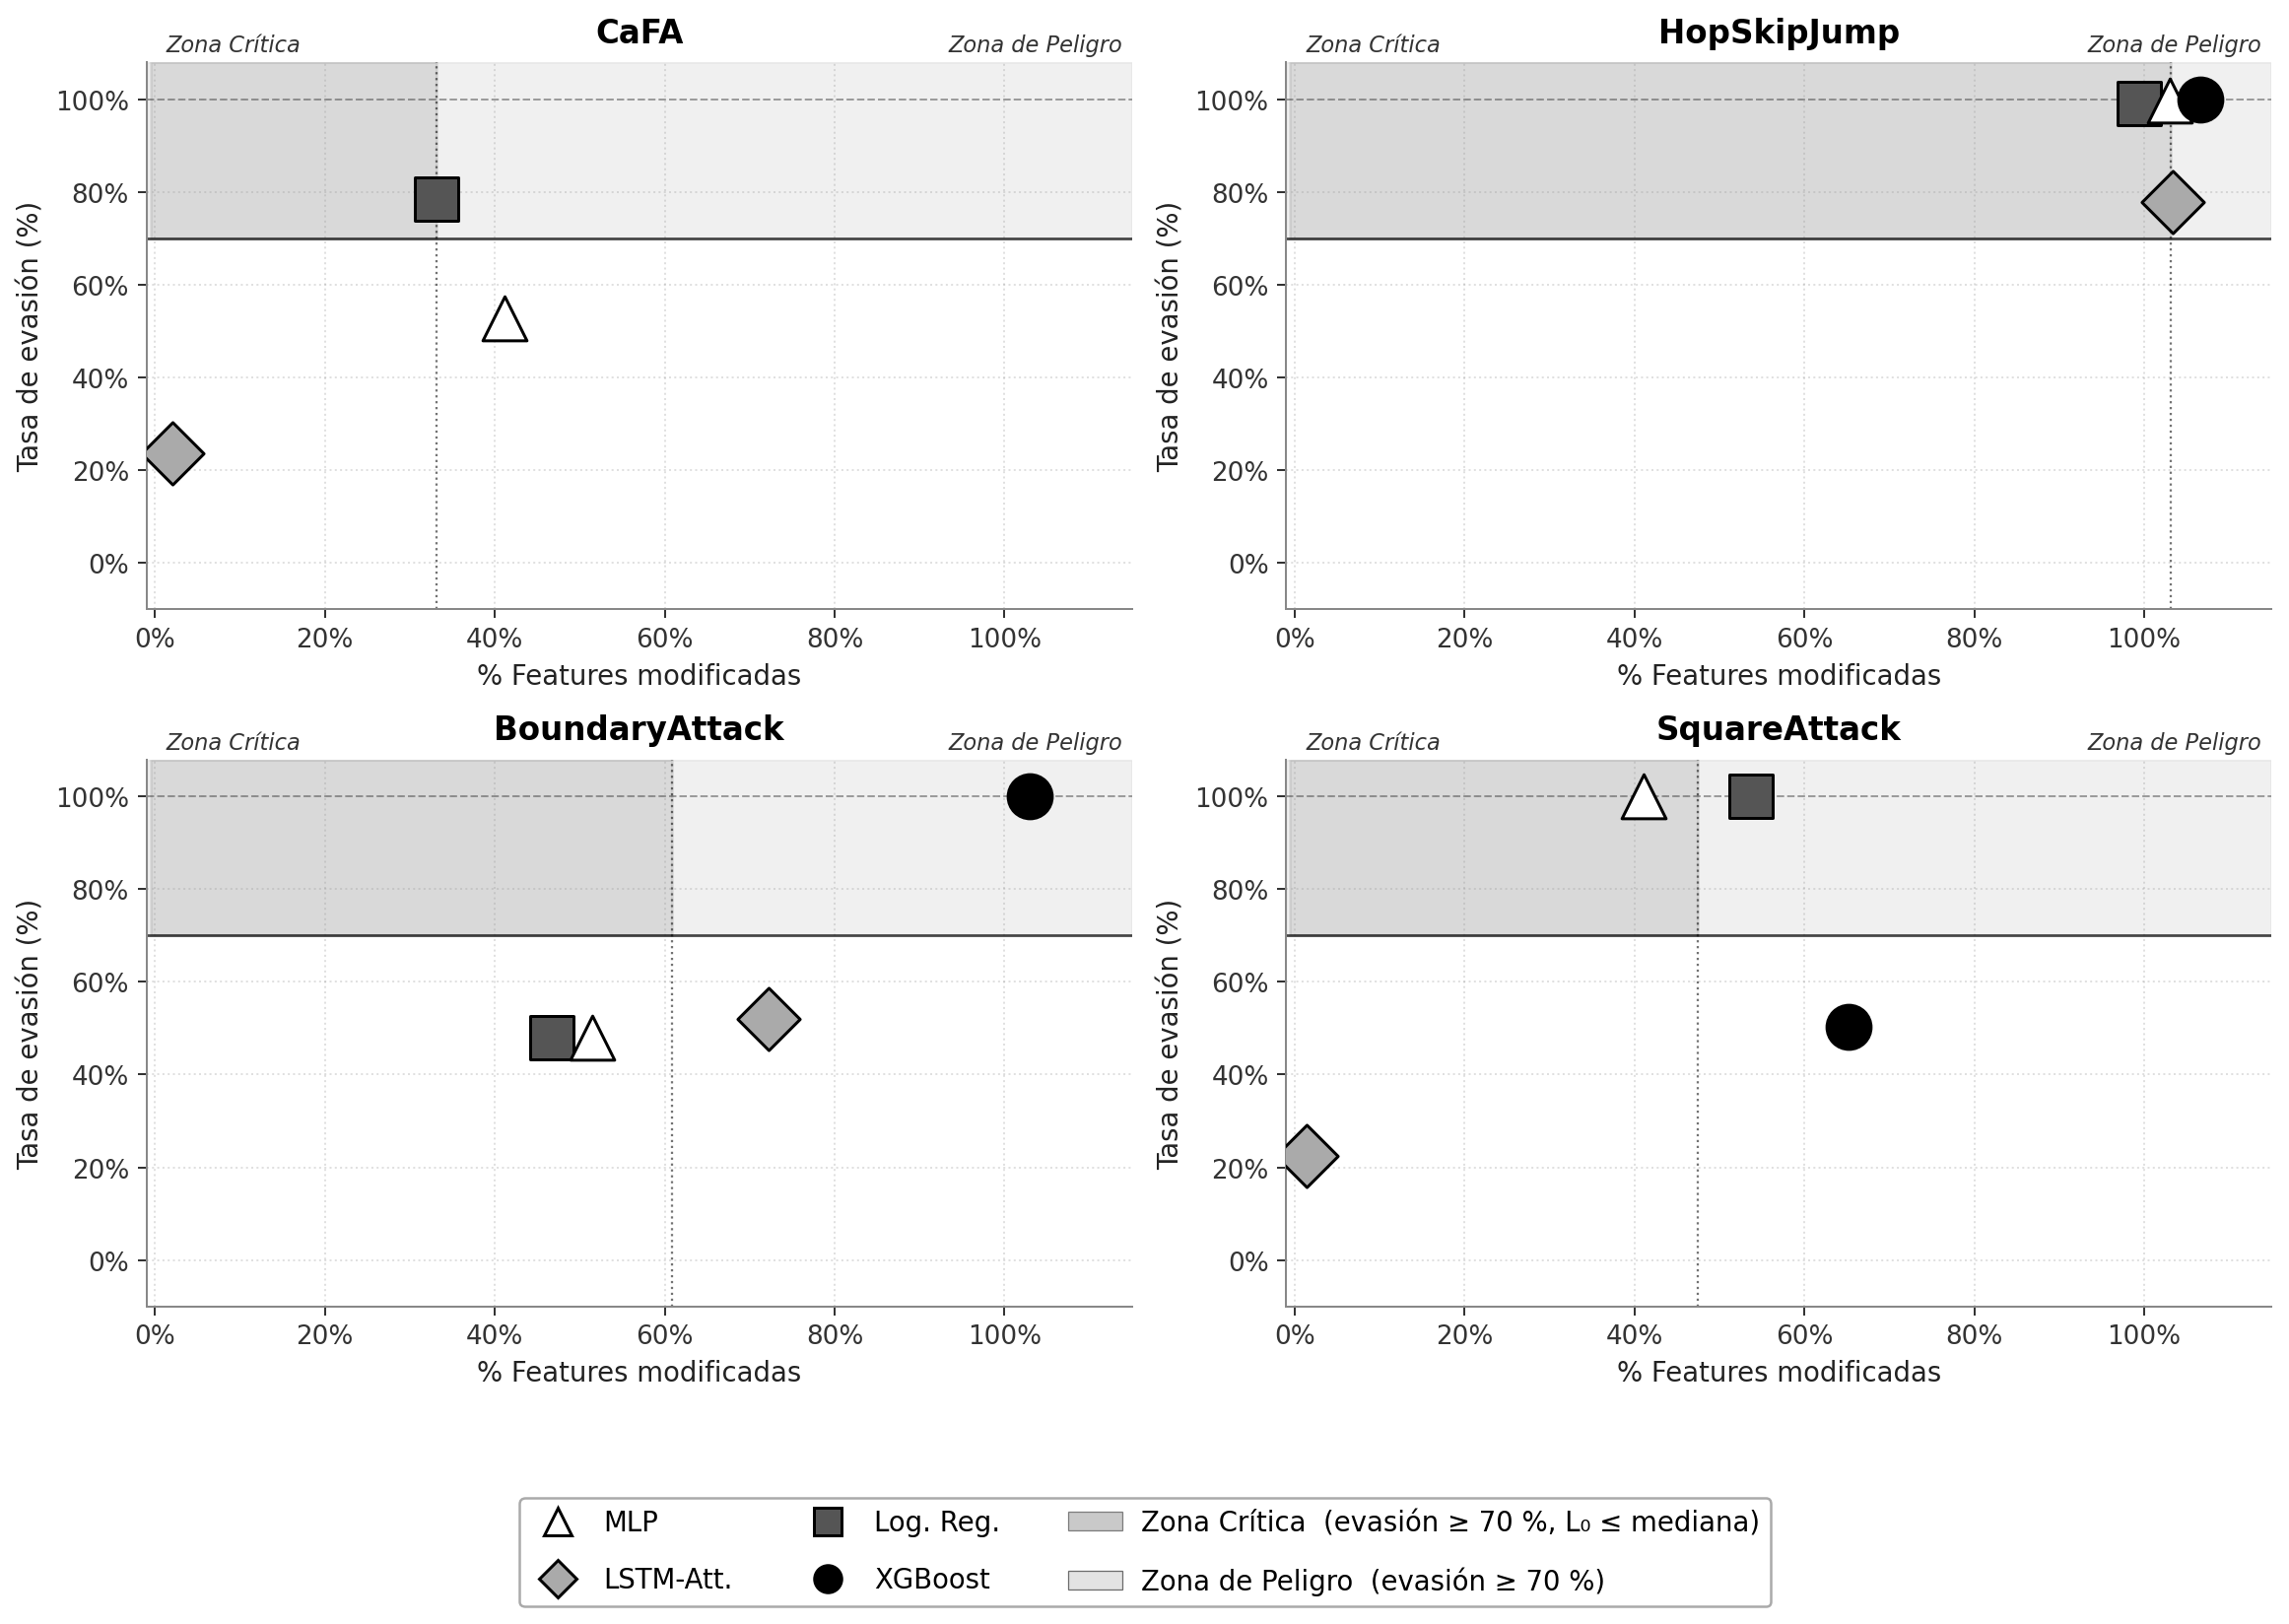
\includegraphics[width=\paperwidth,height=\paperheight,keepaspectratio]{imagenes/bubble_creditcard.png}
\end{frame}

% ── Slide: resumen general Credit Card ──
\begin{frame}{Resumen de Experimentación — Credit Card 2023}
    \begin{columns}
        \column{0.5\textwidth}
        \begin{block}{Condición favorable: Dataset balanceado (50/50)}
            \begin{itemize}
                \item Los \textbf{4 modelos} detectan fraudes correctamente
                \item Recall base $\geq$ 94\% en todos los modelos
                \item Todos son evaluables adversarialmente
            \end{itemize}
        \end{block}

        \vspace{0.3cm}

        \begin{alertblock}{Modelo más vulnerable}
            Log.\ Reg.\ y MLP — evasión total (100\%)
            ante SquareAttack con solo 12--16 features modificadas
        \end{alertblock}

        \column{0.5\textwidth}
        \begin{block}{Resultados de los ataques}
            \begin{itemize}
                \item \textbf{HopSkipJump:} evasión $\approx$99\% en todos
                los modelos, pero modifica $\sim$30 de 29 features
                \item \textbf{SquareAttack:} 100\% sobre MLP y Log.\ Reg.\
                con solo 12--16 features — mayor amenaza real
                \item \textbf{CaFA:} evasión moderada (24--78\%)
                con muy pocas features ($L_0 < 12$)
                \item \textbf{LSTM-Att.} es el modelo más robusto
            \end{itemize}
        \end{block}

        \vspace{0.3cm}

        \begin{exampleblock}{Conclusión}
            Alto rendimiento base \textbf{no implica}
            robustez adversarial — todos los modelos
            son vulnerables a al menos 2 ataques.
        \end{exampleblock}
    \end{columns}
\end{frame}


% ── Slide: Gráfico de burbujas — AMLworld sin SMOTE ──
\begin{frame}[plain]
    \centering
    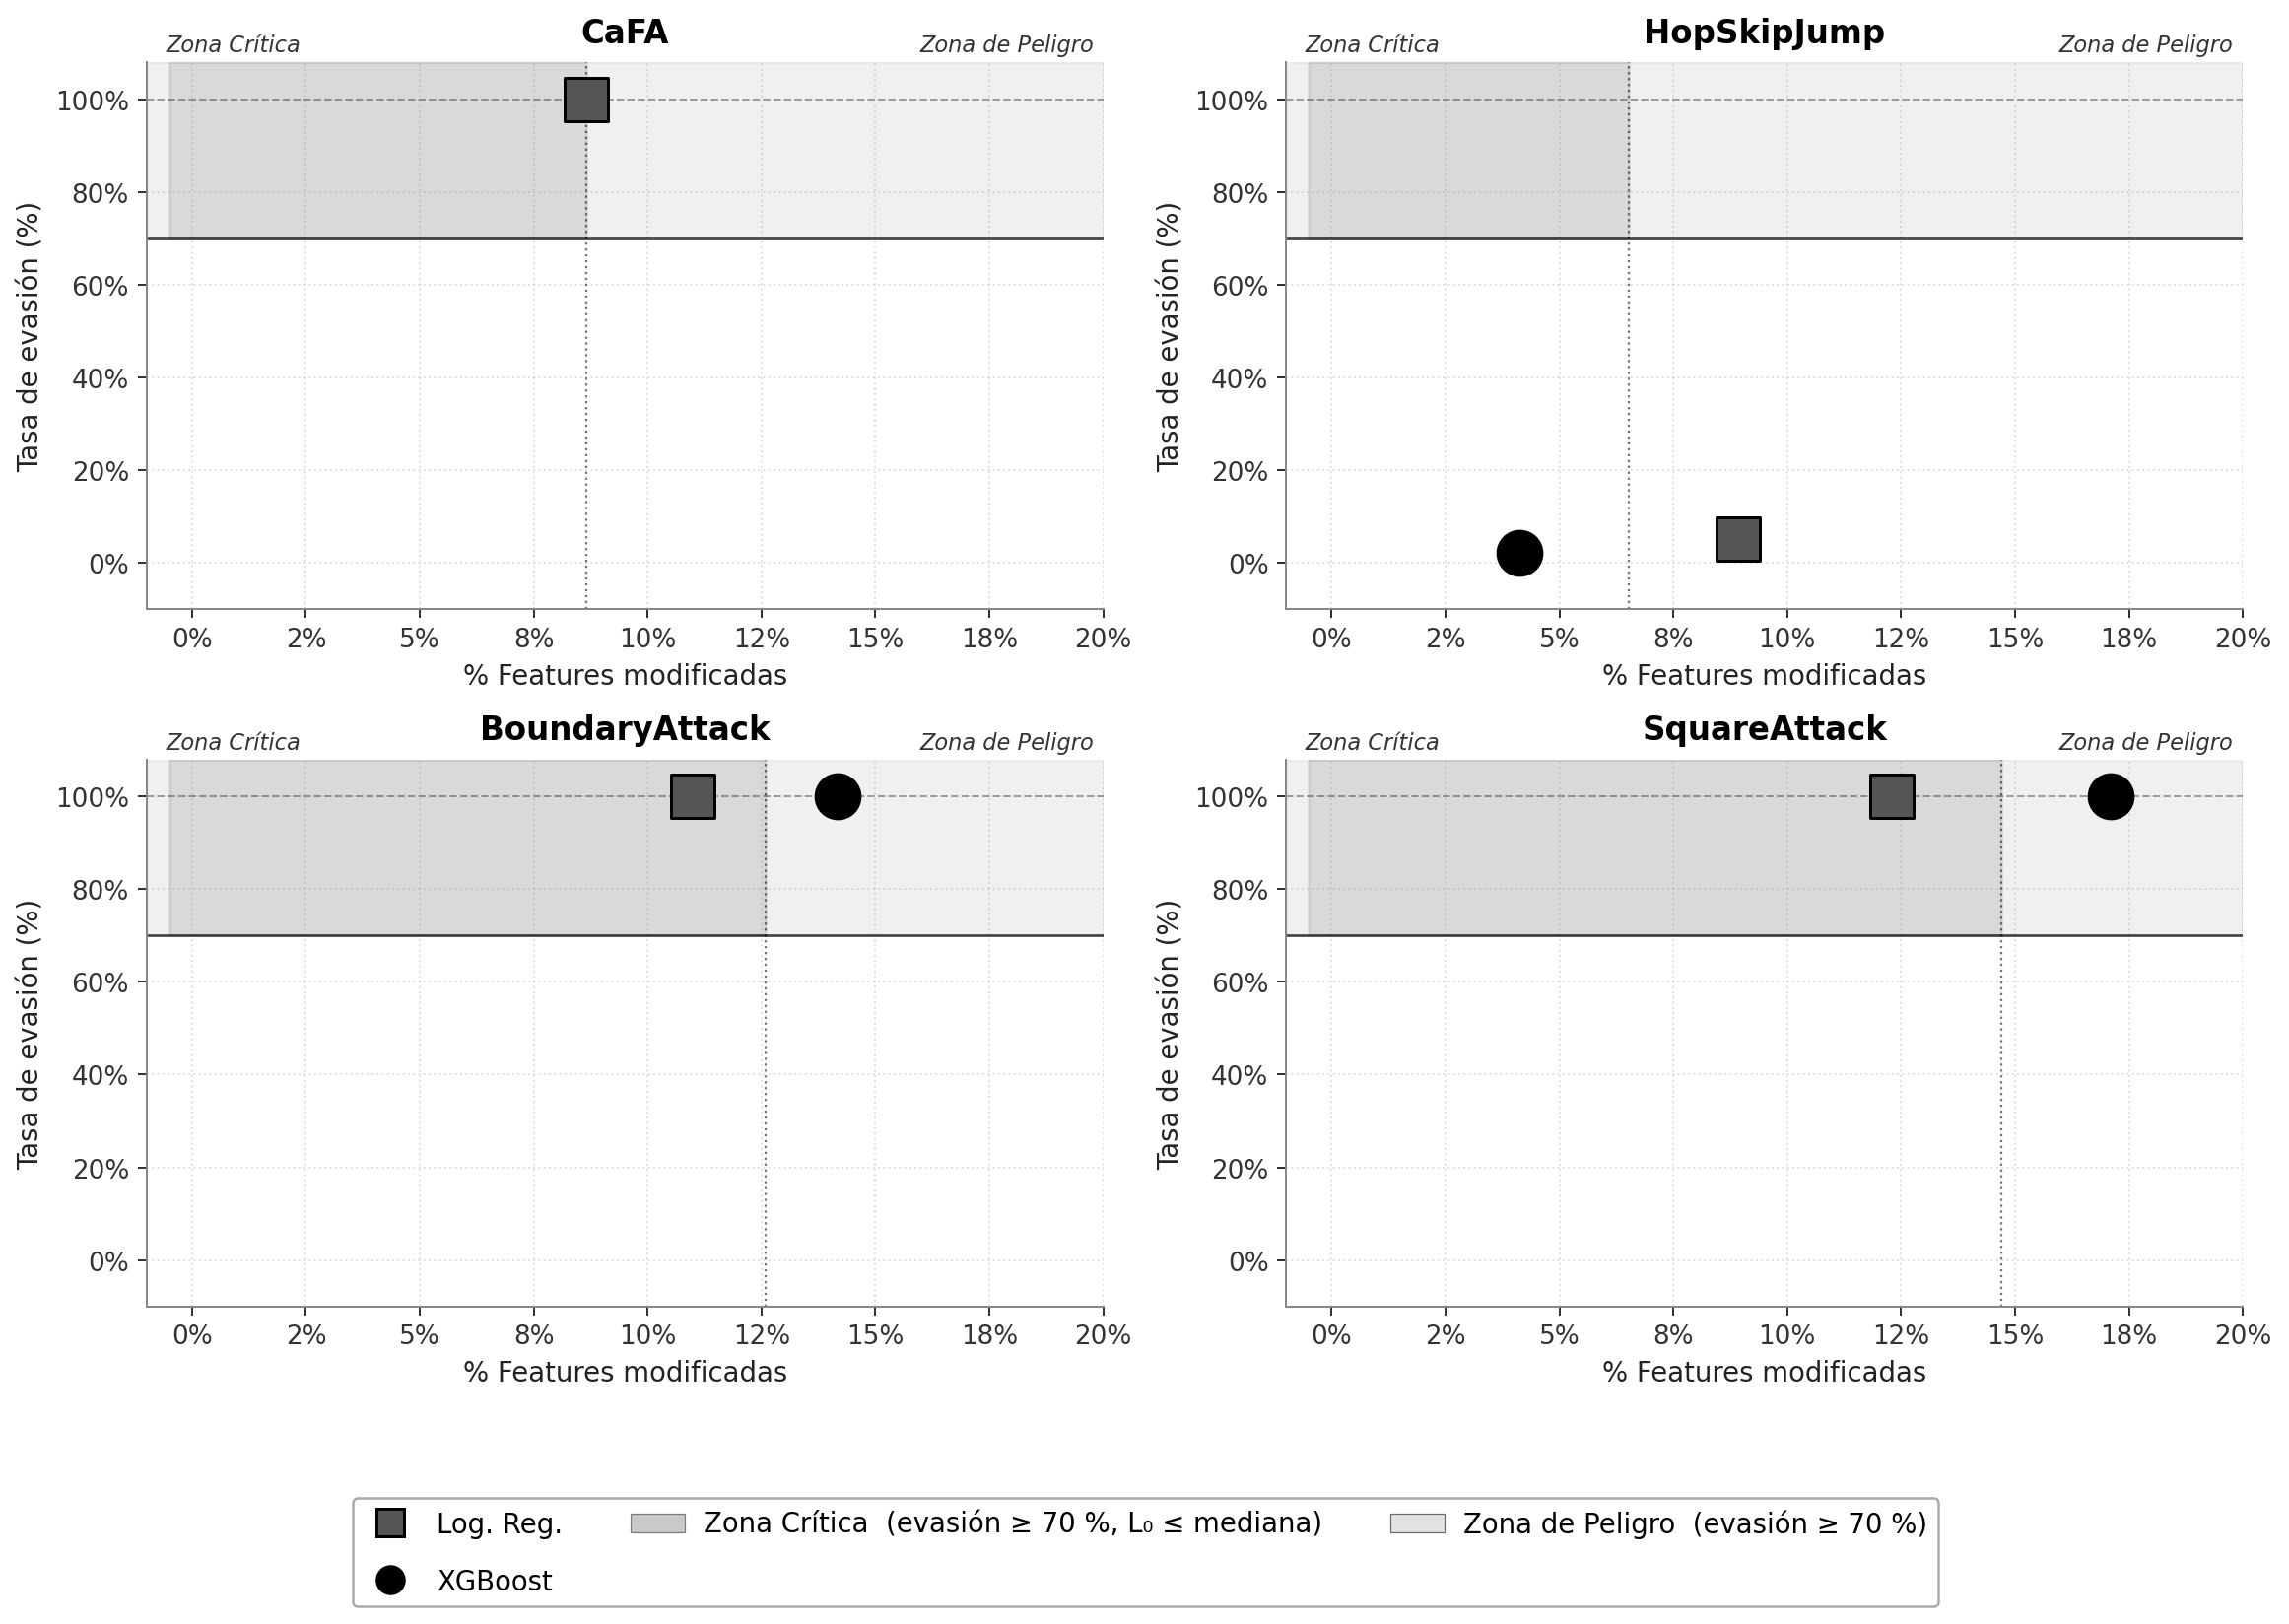
\includegraphics[width=\paperwidth,height=\paperheight,keepaspectratio]{imagenes/bubble_amlworld.png}
\end{frame}



% ── Slide: resumen general AMLworld ──
\begin{frame}{Resumen de Experimentación — AMLworld HI-Small}
    \begin{columns}
        \column{0.5\textwidth}
        \begin{alertblock}{Problema: Imbalance 1:979}
            \begin{itemize}
                \item MLP y LSTM-Att.\ colapsan a Recall = 0\%
                \item Solo \textbf{XGBoost} y \textbf{Log.\ Reg.}\ detectan fraudes
                \item Sin detección base → no hay nada que atacar
            \end{itemize}
        \end{alertblock}

        \vspace{0.3cm}

        \begin{block}{Modelos evaluables adversarialmente}
            \begin{itemize}
                \item XGBoost — Recall base: 33.95\%
                \item Log.\ Reg. — Recall base: 10.67\%
            \end{itemize}
        \end{block}

        \column{0.5\textwidth}
        \begin{block}{Resultados de los ataques}
            \begin{itemize}
                \item \textbf{3 de 4 ataques} logran evasión total (100\%)
                modificando solo \textbf{3--6 de 41 features codificadas}
                \item \textbf{HopSkipJump} es el único ataque resistido
                ($\leq$5.2\% evasión)
                \item \textbf{CaFA} incompatible con XGBoost
                (requiere gradientes)
            \end{itemize}
        \end{block}

        \vspace{0.3cm}

        \begin{exampleblock}{Conclusión}
            Un atacante solo necesita modificar
            3--6 campos de una transacción para
            evadir completamente la detección.
        \end{exampleblock}
    \end{columns}
\end{frame}

% ── Slide: Gráfico de burbujas — AMLworld con SMOTE ──
\begin{frame}[plain]
    \centering
    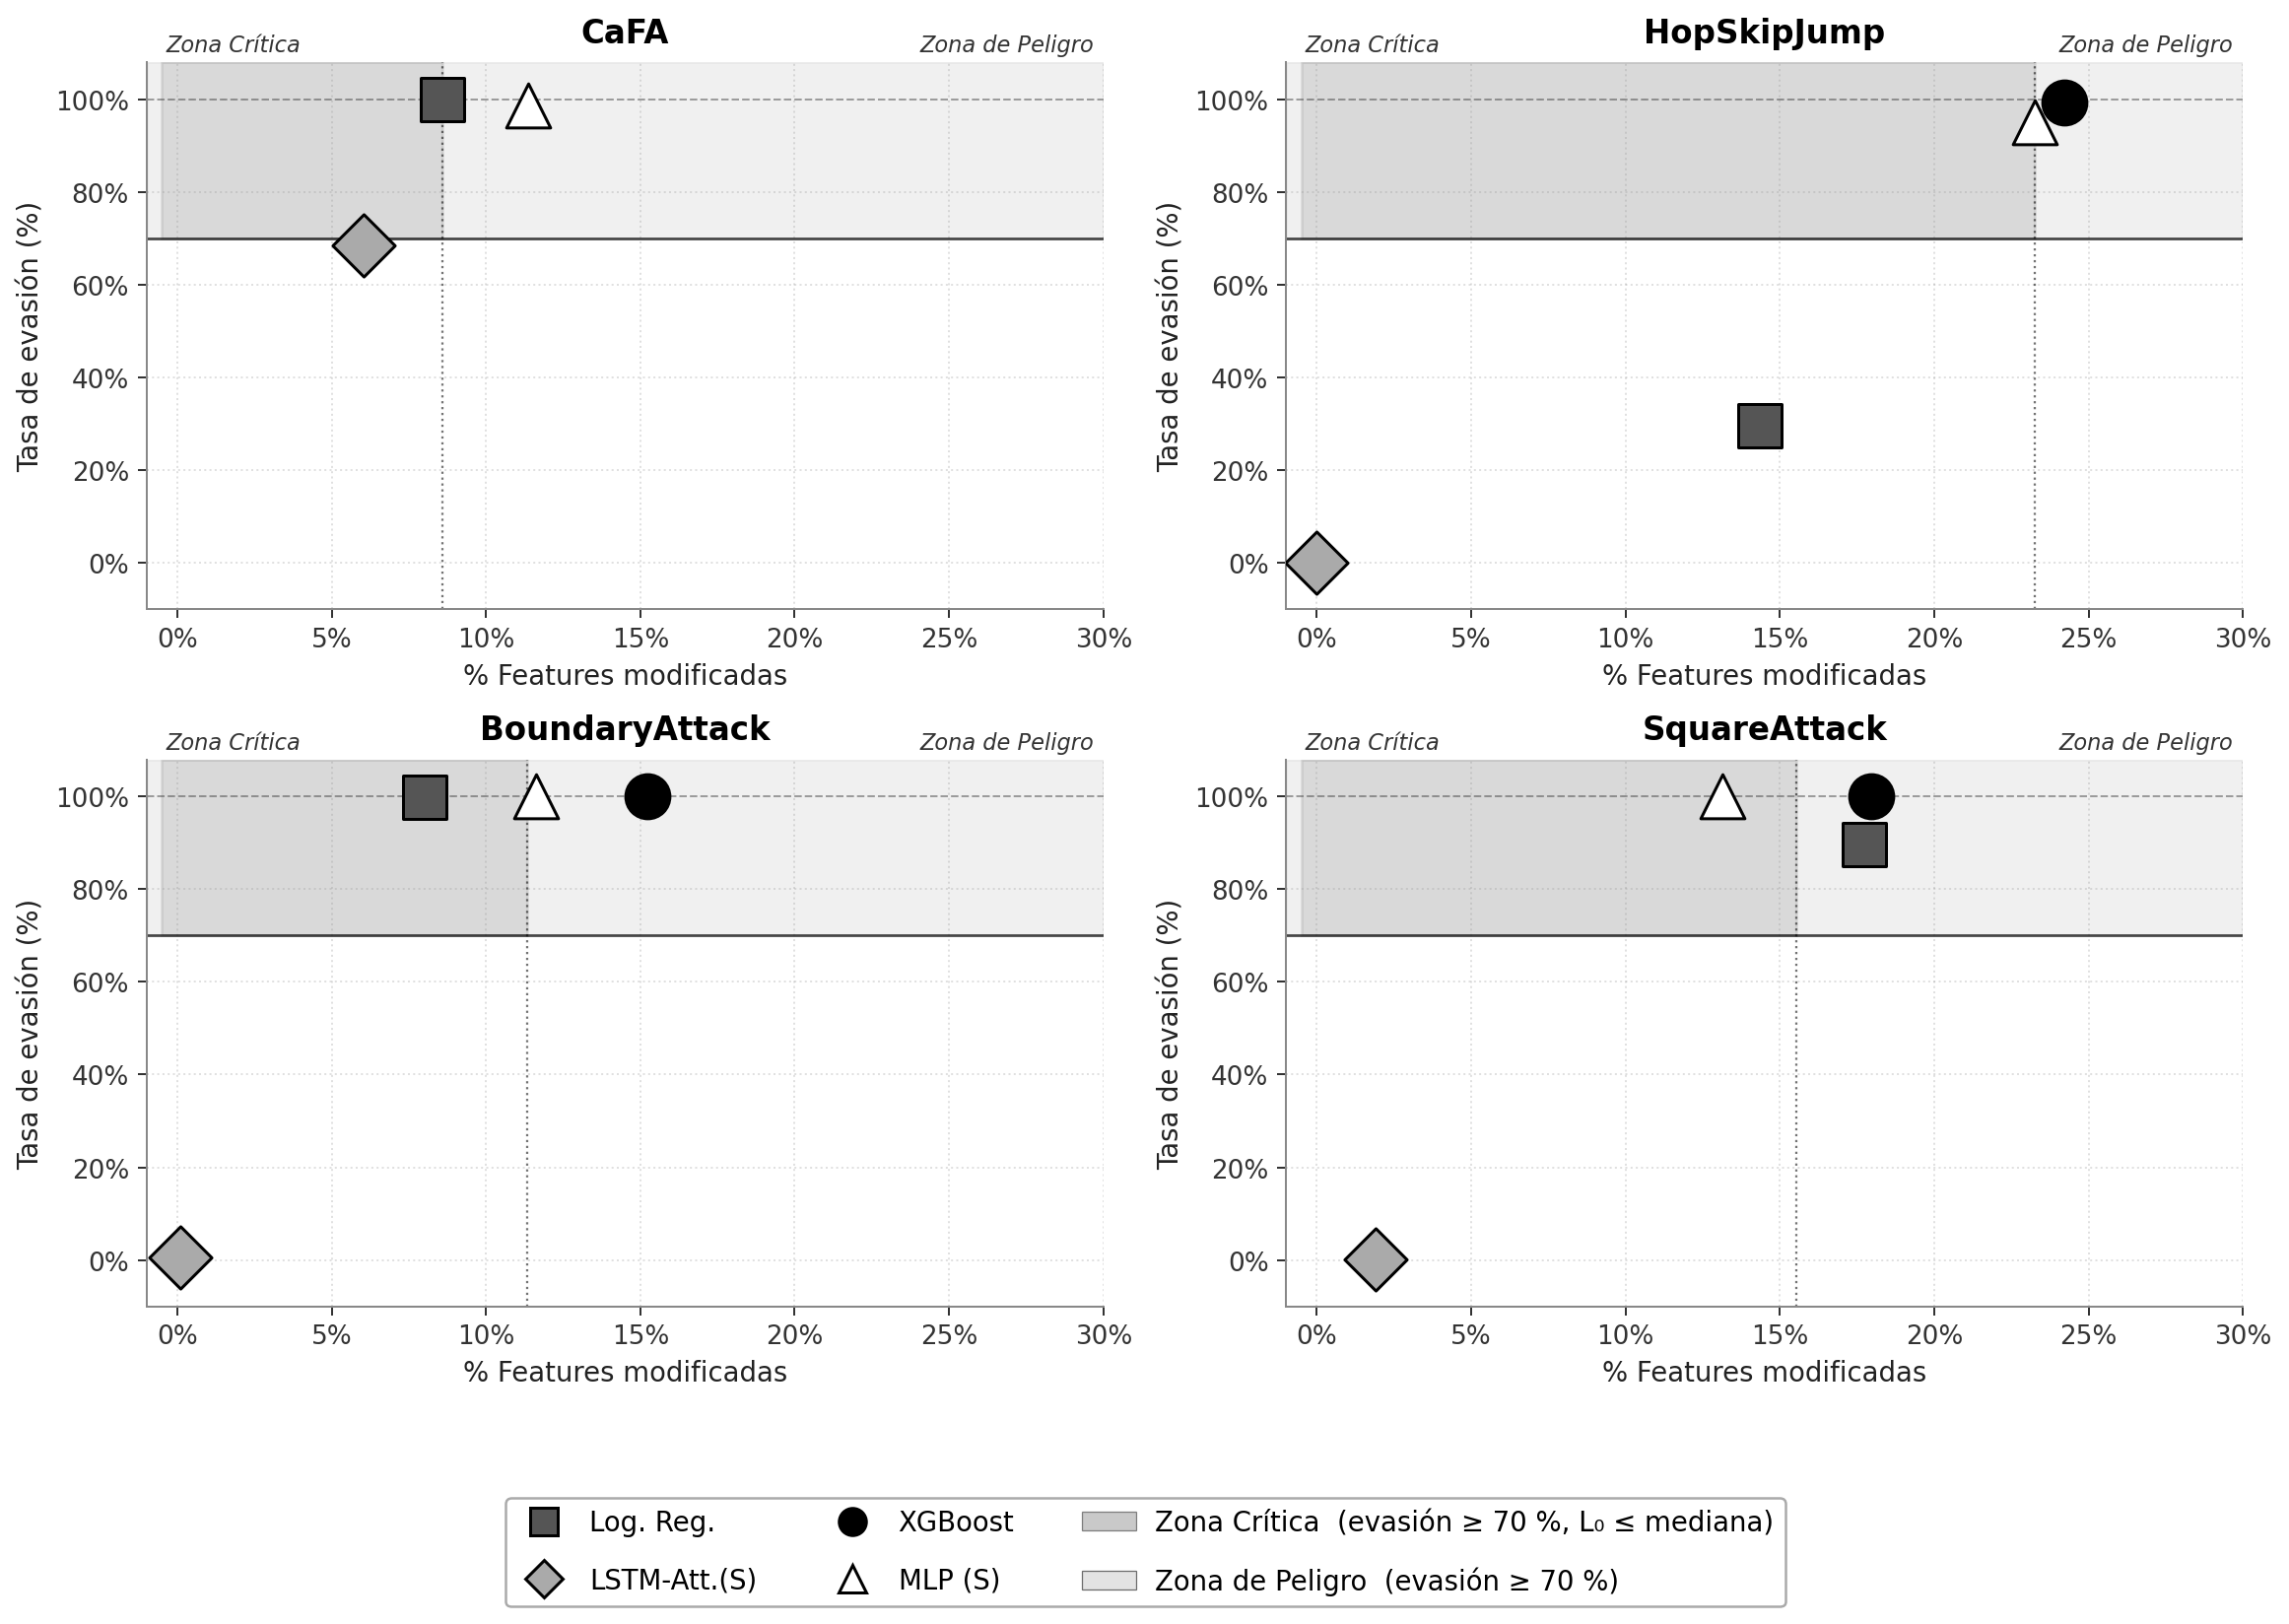
\includegraphics[width=\paperwidth,height=\paperheight,keepaspectratio]{imagenes/bubble_amlworld_smote.png}
\end{frame}

% ── Slide: resumen AMLworld con SMOTE ──
\begin{frame}{Resumen de Experimentación — AMLworld con SMOTE}
    \begin{columns}
        \column{0.5\textwidth}
        \begin{exampleblock}{SMOTE habilita 4 modelos evaluables}
            \begin{itemize}
                \item XGBoost y Log.\ Reg.\ mejoran notablemente
                \item MLP\,(S) y LSTM-Att.\,(S) ahora detectan fraudes
                \item Zona de Peligro: \textbf{71\,\%} de las combinaciones
                ($\uparrow$ vs 53\,\% en Credit Card)
            \end{itemize}
        \end{exampleblock}

        \vspace{0.3cm}

        \begin{alertblock}{Modelo más vulnerable}
            MLP\,(S) — evasión $\geq$95\,\% ante los 4 ataques
            modificando menos del 24\,\% de features
        \end{alertblock}

        \column{0.5\textwidth}
        \begin{block}{Hallazgo clave: Paradoja de robustez}
            \begin{itemize}
                \item \textbf{LSTM-Att.\,(S)} resiste 3 de 4 ataques
                ($\leq$0.5\,\% evasión ante ataques de caja negra)
                \item Razón: sesgo hacia fraude + frontera de
                decisión irregular por LSTM + atención
                \item \textbf{Robustez adversarial $\neq$ utilidad operacional}
            \end{itemize}
        \end{block}

        \vspace{0.3cm}

        \begin{exampleblock}{Conclusión}
            SMOTE amplía la superficie de ataque
            pero también revela modelos robustos
            que no serían evaluables sin balanceo.
        \end{exampleblock}
    \end{columns}
\end{frame}

% ---------------------------------------------------------
% CAPÍTULO 06: CONCLUSIONES
% ---------------------------------------------------------
\begin{frame}
\vfill
\centering
{\fontsize{28}{34}\selectfont\bfseries CONCLUSIONES}
\vfill
\end{frame}
\section{Conclusiones y Trabajo Futuro}

% ---------------------------------------------------------
% CAPÍTULO 06 - PÁGINA 01
% ---------------------------------------------------------
\begin{frame}{Conclusiones y Proyecciones}
    \begin{block}{Conclusiones Fundamentales}
        \begin{enumerate}
            \item \textbf{Alto rendimiento base no implica robustez:} Los modelos con métricas óptimas colapsan ante perturbaciones sutiles — el 53\,\% (CC) y 71\,\% (AMLworld) de las combinaciones caen en \textbf{Zona de Peligro} (evasión $\geq$70\,\%).
            \item \textbf{SMOTE: condición necesaria y amplificador de riesgo:} Sin balanceo, MLP y LSTM-Att.\ son inútiles para detección \emph{y} para evaluación adversarial. Con SMOTE, el 71\,\% de las combinaciones quedan expuestas.
            \item \textbf{Paradoja de robustez:} LSTM-Att.\,(S) resiste 3 de 4 ataques de caja negra ($\leq$0.5\,\% evasión), pero su F1\,=\,0.25\,\% lo hace inoperable en producción. \textbf{Robustez adversarial $\neq$ utilidad operacional.}
            \item \textbf{$L_0$ como métrica de sigilo:} AMLworld permite evasión total modificando $<$15\,\% de las features; la Zona Crítica identifica los ataques más peligrosos de manera comparable entre datasets.
        \end{enumerate}
    \end{block}

    \vspace{0.15cm}
    \begin{exampleblock}{Siguientes Pasos}
        \begin{itemize}
            \item \textbf{Defensa basada en $L_0$:} alertar cuando múltiples features cambian simultáneamente en una transacción.
            \item \textbf{Entrenamiento adversarial:} incorporar ejemplos adversariales para aumentar la robustez sin sacrificar F1.
            \item \textbf{Transferibilidad:} evaluar si ataques sobre un modelo impactan a modelos desconocidos (ataques de caja negra transferibles).
        \end{itemize}
    \end{exampleblock}
\end{frame}


% ---------------------------------------------------------
% CAPÍTULO 06 - PÁGINA 02
% ---------------------------------------------------------
\begin{frame}{Referencias Principales}
\footnotesize
\begin{itemize}
    \item Altman, E. et al. (2024). Realistic Synthetic Financial Transactions for Anti-Money Laundering Models. \textit{NeurIPS Datasets and Benchmarks Track}.
    \item Cartella, F. et al. (2021). Adversarial Attacks on Tabular Data in Financial Fraud Detection. \textit{ACM International Conference on AI in Finance}.
    \item Chen, J. et al. (2019). HopSkipJumpAttack: A query-efficient decision-based attack. \textit{IEEE Symposium on Security and Privacy}.
    \item Dyrmishi, S. et al. (2025). Adversarial Attacks and Defenses on Tabular Data: A Systematic Survey. \textit{arXiv preprint}.
\end{itemize}
\end{frame}

% ---------------------------------------------------------
% CAPÍTULO 06 - PÁGINA 03
% ---------------------------------------------------------
\begin{frame}
    \centering
    \Huge \textbf{¡Muchas Gracias!}

    \vspace{1cm}
    \normalsize
    Javier Chavarria \& Alejandro Chipayo \\
    \vspace{0.2cm}
    \footnotesize{Ciencia de la Computación --- UTEC}
\end{frame}

\end{document}
